\documentclass{GZUbachelorthesis}
\titlepageset{
    title = {贵州大学本科毕业论文 \LaTeX 模板使用示例文档}, %论文标题,可用\\手动分行
    title* = {An Example Appling \LaTeX\ Template for\\Bachelor Thesis of Guizhou University}, %论文英文标题
    department = {数学与统计学院}, %学院
    major = {数学与应用数学}, %专业
    majorcode = {070101}, %专业代码
    class = {应数0001}, %班级
    studentID = {1234567890}, %学号
    author = {叶致豪}, %作者姓名
    author* = {Ye Zhi-Hao}, %作者英文姓名
    teacher = {李思锐}, %指导老师
    date = {2025年2月18日}, %日期
}
\graphicspath{{figures/}} %定义所插入的图片均在figures文件夹内

\begin{document}
\maketitle %生成封面页和诚信责任书

\begin{tocabstract} %生成目录和摘要
\begin{abstract}[关键词一;关键词二;关键词三;关键词四] %中文摘要
    首先声明：本模板不是贵州大学官方层面发布的指定模板，使用本模板前请务必核对学校官方在该年的具体格式要求，并与自己的导师交流，确认无误后才可应用。本项目开源，采用\href{https://www.latex-project.org/lppl/lppl-1-3c/}{\LaTeX 项目公共许可证v1.3}授权协议，若因使用本模板引起纠纷，模板的所有制作者概不负责。

    \textbf{强烈建议具备一定 \LaTeX 使用经验后再来使用本模板。}

    题目应简洁、明确、有概括性,字数不宜超过20个字.摘要要有高度的概括力,语言精练、明确.扼要叙述论文的主要内容、方法、成果和结论.摘要中不宜使用公式、图表,不标注引用文献编号.同时要有中、英文对照摘要,中文摘要约300\~{}500字.关键词从论文标题或正文中挑选3\~{}5个最能表达主要内容的词作为关键词,同时有中、英文对照,分别附于中、英文摘要后.目录一般按三级标题编写,要求标题层次清晰.目录中标题应与正文中标题一致.
\end{abstract}
\begin{enabstract}[keyword 1; keyword 2; keyword 3; keyword 4] %英文摘要
  Statement: This template is not officially released by Guizhou University. Before using it, you must thoroughly verify the specific formatting requirements issued by the university for that academic year and discuss it with your supervisor. Only after confirming their accuracy can this template be applied. This project is licensed under the \href{https://www.latex-project.org/lppl/lppl-1-3c/}{The LaTeX project public license v1.3c}.There is no warranty for your thesis. Should the thesis prove defective, you assume the cost of all necessary servicing, repair, or correction.

  \textbf{It is strongly suggested that users acquire prior experience with LaTeX before utilizing this template.}

  The title should be concise, clear, and comprehensive, preferably within 20 words. The abstract requires a high degree of conciseness, using precise and clear language. It should succinctly outline the main content, methodology, findings, and conclusions of the paper. Formulas, charts, and reference citation numbers should not be included in the abstract. Both Chinese and English abstracts are required.Select 3-5 keywords that best represent the main content from the paper's title or body text. Both Chinese and English keywords are required and should be placed after their respective abstracts.The TOC is generally organized using a three-level heading system, ensuring clear hierarchical structure. The headings in the TOC must correspond exactly to the headings used in the main text.
\end{enabstract}
\end{tocabstract}

\section{毕业论文主要部分的撰写}
毕业论文（设计），必须由学生本人独立完成，不得弄虚作假，不得抄袭他人成果或使用AI工具代写。

毕业论文（设计）应中心突出，内容充实，论据充分，论证有力，数据可靠，结构紧凑，层次分明，图表清晰，格式规范，文字流畅，字迹工整，结论正确。

毕业论文的字数，人文社科类专业原则上不少于1万字，理工农医类专业不少于1.2万字。对于部分专业毕业设计成果由毕业设计图纸和毕业论文两部分组成者，其毕业论文字数原则上应不低于0.8万字。作品阐释类原则上不低于0.5万字。各专业可根据具体情况适当调整。调整较大的需报教务处备案。

\subsection{引言的写法}
一篇学位论文的引言大致包含如下几个部分：1、问题的提出；2、选题背景及意义；3、文献综述；4、研究方法；5、论文结构安排。
\begin{itemize}
  \item 问题的提出：要清晰地阐述所要研究的问题“是什么”。
    \footnote{选题时切记要有“问题意识”，不要选不是问题的问题来研究。}
  \item 选题背景及意义：论述清楚为什么选择这个题目来研究，即阐述该研究对学科发展的贡献、对国计民生的理论与现实意义等。
  \item 文献综述：对本研究主题范围内的文献进行详尽的综合述评，“述”的同时一定要有“评”，指出现有研究状态，仍存在哪些尚待解决的问题，讲出自己的研究有哪些探索性内容。
  \item 研究方法：讲清论文所使用的学术研究方法。
  \item 论文结构安排：介绍本论文的写作结构安排。
\end{itemize}

\subsection{正文的写法}
本部分是论文作者的研究内容，不能将他人研究成果不加区分地掺和进来。已经在引言的文献综述部分讲过的内容，这里不需要再重复。各章之间要存在有机联系，符合逻辑顺序。

\subsection{结论的写法}
结论是对论文主要研究结果、论点的提炼与概括，应精炼、准确、完整，使读者看后能全面了解论文的意义、目的和工作内容。结论是最终的、总体的结论，不是正文各章小结的简单重复。结论应包括论文的核心观点，主要阐述作者的创造性工作及所取得的研究成果在本领域中的地位、作用和意义，交代研究工作的局限，提出未来工作的意见或建议。同时，要严格区分自己取得的成果与指导教师及他人的学术成果。

在评价自己的研究工作成果时，要实事求是，除非有足够的证据表明自己的研究是“首次”、“领先”、“填补空白”的，否则应避免使用这些或类似词语。

\subsection{参考文献和致谢的写法}
参考文献是毕业论文（设计）不可缺少的组成部分，它反映论文作者的科学态度和毕业论文（设计）的取材来源、广博程度和可靠程度，同时能方便地把作者的研究成果与他人的成果区别开来。一份完整的参考文献也是向读者提供的一份有价值的信息资料。一般做毕业论文（设计）的参考文献不宜过多，但应列入主要的中外文献。

致谢即以简短的文字对课题研究与论文撰写过程中曾直接给予帮助的指导教师、答疑教师及其他人员表示自己的谢意。

\clearpage %每章/节之间要求分页
\section{图表的插入示例}
文中图、表只用中文图题、表题。对于函数曲线图，请注意检查横纵坐标的变量名、单位、刻度值是否完整（对于无量纲化或无单位的，请注明“无单位”），不同线型或图符说明应完整，变量名和单位之间用“/”分开。表的宽度不得超过版面文字的宽度，表一律要求采用三线表，表中参数及单位用“/”分开。

\subsection{图的插入示例}
每幅插图应有图序和图题，图序和图题应放在图位下方居中处，图序和图题一般用黑体五号字。图的编号由“图”和阿拉伯数字组成，阿拉伯数字由前后两部分组成，中间用“.”号分开，前部分数字表示图所在章的序号，后部分数字表示图在该章的序号。例如“图2.3”；每个图号后面都必须有图题，图的编号和图题要置于图下方的居中位置。

建议矢量图片使用 PDF 格式，比如数据可视化的绘图；照片应使用 JPG 格式；其他栅格图应使用无损的 PNG 格式。注意，LaTeX 不支持 TIFF 格式；EPS 格式已经过时。

\begin{figure}[h]
  \centering
  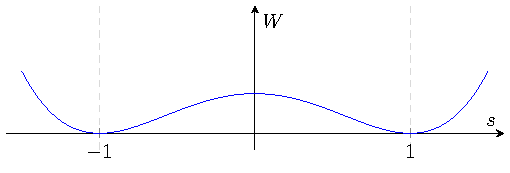
\includegraphics[width=0.5\linewidth]{figure-function.pdf} %图片宽度为0.5倍行宽
  \caption{函数图象的示例}
  \label{fig:function}
\end{figure}

如果一个图由两个或两个以上分图组成时，各分图分别以(a)，(b)，(c)……作为图序，并须有分图题。

\begin{figure}[h]
  \centering
  \subcaptionbox{分图A的示例\label{fig:subfig-a}}
    {
\includegraphics[width=0.35\linewidth]{image-a.pdf}} %图片宽度为0.35倍行宽
  \subcaptionbox{分图B的示例\label{fig:subfig-b}}
    {
\includegraphics[width=0.35\linewidth]{image-b.pdf}} %图片宽度为0.35倍行宽
  \caption{多个分图的示例}
  \label{fig:multi-image}
\end{figure}

\subsection{表的插入示例}
每个表格应有自己的表序和表题，一般用黑体五号字，表的编号方法同图的编号方法相同，例如“表1.6”，“表2.3”等；表的编号和表题要置于表上方的居中位置。

\begin{table}[ht]
  \centering
  \caption{三线表的示例}
  \begin{tabular}{cc}
    \toprule
    文件名 & 描述 \\
    \midrule
    GZUbachelorthesis.cls & 模板文件 \\
    example.pdf & 应用了模板的示例文档 \\
    example.tex & 应用了模板的示例文档的源文件 \\
    examplebib.bib & 示例文档的参考文献库 \\
    \bottomrule
  \end{tabular}
  \label{tab:three-line}
\end{table}

如某个表需要转页接排，在随后的各页上要重复表的编号，编号后跟表题（可省略）或跟“（续）”，如“表1.2（续）”。续表均要重复表的编排。

\begin{longtable}[ht]{cccc}
    \caption{跨页长表格的示例}
    \label{tab:longtable} \\
    \toprule
    表头 1 & 表头 2 & 表头 3 & 表头 4 \\
    \midrule
  \endfirsthead
    \caption*{表~\thetable（续）} \\
    \toprule
    表头 1 & 表头 2 & 表头 3 & 表头 4 \\
    \midrule
  \endhead
    \bottomrule
  \endfoot
  Row 1  & & & \\
  Row 2  & & & \\
  Row 3  & & & \\
  Row 4  & & & \\
  Row 5  & & & \\
  Row 6  & & & \\
  Row 7  & & & \\
  Row 8  & & & \\
  Row 9  & & & \\
  Row 10 & & & \\
  Row 11  & & & \\
  Row 12  & & & \\
  Row 13  & & & \\
  Row 14  & & & \\
  Row 15  & & & \\
  Row 16  & & & \\
  Row 17  & & & \\
  Row 18  & & & \\
  Row 19  & & & \\
  Row 20 & & & \\
\end{longtable}

\subsection{算法伪代码的插入示例}
给定字符集$C = \{x_1,x_2,\cdots,x_n\}$和每个字符的频率$f(x_i)$，用Huffman算法构造$C$的一个最优前缀码。
\begin{algorithm}
  \caption{Huffman(C)}
    \KwData{$C = \{x_1,x_2,\cdots,x_n\},\ f(x_i)$.}
    \KwResult{Q. \tcp*[f]{队列}} 
    n $\leftarrow Card(C)$ \;
    Q $\leftarrow C$ \tcp*[r]{按频率递增构成队列Q}

    \For{i $\leftarrow 1$ \KwTo n-1}{
      z $\leftarrow$ Allocate-Node() \tcp*[r]{生成结点z}
      x $\leftarrow \min{Q}$ \;
      z.left $\leftarrow$ x \tcp*[r]{取Q中最小元作z的左儿子}
      y $\leftarrow \min{Q\backslash\{x\}}$ \; 
      z.right $\leftarrow$ y \tcp*[r]{取Q中第二小元作z的右儿子}
      $f(z) \leftarrow f(x)+f(y)$ \;
      Insert(Q,z) \tcp*[r]{将z插入Q}
    }
    \KwRet{Q} \;
\end{algorithm}

\clearpage %每章/节之间要求分页
\section{总结与展望}
本模板还有许多可改进的地方，同时本项目也需要长期的维护以便适应学校每一年不同的论文格式要求。希望能有志同道合的校友愿意加入这个开源的项目。

\nocite{卡德斯图赛1996,李思锐2015} %文中未引用但需要列出的文献
\bibliography{examplebib} %参考文献

\thanks %致谢
本文是在李思锐教授的指导下完成的。毕业之际，我首先要感谢的便是李老师。……

其次，我还要感谢……

最后,感谢父母和家人对我的支持鼓励。你们无私的爱，是我一生的精神财富。

\appendix %附录
对于一些不宜放入正文中、但作为毕业论文（设计）又不可或缺的组成部分或具有重要参考价值的内容，可编入毕业论文（设计）的附录中，例如，公式的推演、编写的算法语言程序等。如果毕业论文（设计）中引用的实例、数据资料，实验结果等符号较多时，为了节约篇幅，便于读者查阅，可以编写一个符号说明，注明符号代表的意义。附录的篇幅不宜太多，附录一般不要超过正文。毕业设计的各种图纸、数据表格、计算机程序等材料可作为附录。

\subsection*{积分中值定理例题}
% 除了下面的lem引理环境，模板还预先定义了thm定理环境
\begin{lem}\label{lem:integral mean value example}
    设$f(x) \in C[0,2],\ f(x) > 0,\ a_n = \int_{0}^{2}x^nf(x)\mathrm{d}x$,那么$\sum\limits_{n=0}^{\infty}\frac{x^n}{a_n}$的收敛域为$(-2,2)$.
\end{lem}
在附录给出引理\ref{lem:integral mean value example}的证明.
\begin{proof}
    由第一积分中值定理,\ $\exists \xi \in [0,2]s.t.$
    \[
        a_n = \int_{0}^{2}x^nf(x)\mathrm{d}x = f(\xi)\int_{0}^{2}x^n\mathrm{d}x = f(\xi)\frac{2^{n+1}}{n+1}.
    \]
    由Cauchy-Hadamard定理,
    \[
        \varlimsup_{n\to\infty} \sqrt[n]{\left|\frac{1}{a_n}\right|} = \varlimsup_{n\to\infty} \sqrt[n]{\frac{n+1}{f(\xi)}}\sqrt[n]{\frac{1}{2^{n+1}}} = \frac{1}{2},
    \]
    幂级数收敛半径为2.

    分别代入$x=2$和$x=-2$,
    \begin{align*}
        \sum_{n=0}^{\infty} \frac{2^n}{a_n} & = \sum_{n=0}^{\infty} \frac{n+1}{2f(\xi)},\\
        \sum_{n=0}^{\infty} \frac{(-2)^n}{a_n} & = \sum_{n=0}^{\infty} \frac{n+1}{2f(\xi)}(-1)^n.
    \end{align*}
    两者均发散.原幂级数的收敛域为$(-2,2)$.
\end{proof}

\subsection*{二阶Runge-Kutta方法}
所编写通用求解函数程序如下所示。
\begin{lstlisting}[language=matlab]
    function [y] = rungekutta2(x,y0,f)
    %rungekutta2 二阶Runge-Kutta方法求解微分方程数值解
    %   x: 待求解点点列
    %   y0: 初始点的函数值
    %   f: 微分方程右端项
    n = length(x);
    y = x; y(1) = y0; %初始化输出函数值
    for i = 1:n-1
        h = x(i+1) - x(i);
        K1 = f(x(i), y(i));
        K2 = f(x(i)+h, y(i)+h*K1);
        y(i+1) = y(i) + 0.5*h*(K1+K2);
    end
\end{lstlisting}

\subsection*{四阶Runge-Kutta方法}
所编写的通用求解函数程序如下所示。
\begin{lstlisting}[language=matlab]
    function [y] = rungekutta4(x,y0,f)
    %rungekutta4 四阶Runge-Kutta方法求解微分方程数值解
    %   x: 待求解点点列
    %   y0: 初始点的函数值
    %   f: 微分方程右端项
    n = length(x);
    y = x; y(1) = y0; %初始化输出函数值
    for i = 1:n-1
        h = x(i+1) - x(i);
        K1 = f(x(i), y(i));
        K2 = f(x(i)+0.5*h, y(i)+0.5*h*K1);
        K3 = f(x(i)+0.5*h, y(i)+0.5*h*K2);
        K4 = f(x(i)+h, y(i)+h*K3);
        y(i+1) = y(i) + h/6 * (K1+2*K2+2*K3+K4);
    end
\end{lstlisting}

\end{document}